\documentclass{standalone}
\usepackage[utf8]{inputenc}
\usepackage{tikz}
\usepackage{amsmath}
\usepackage{amsfonts}
\usepackage{amssymb}
\begin{document}

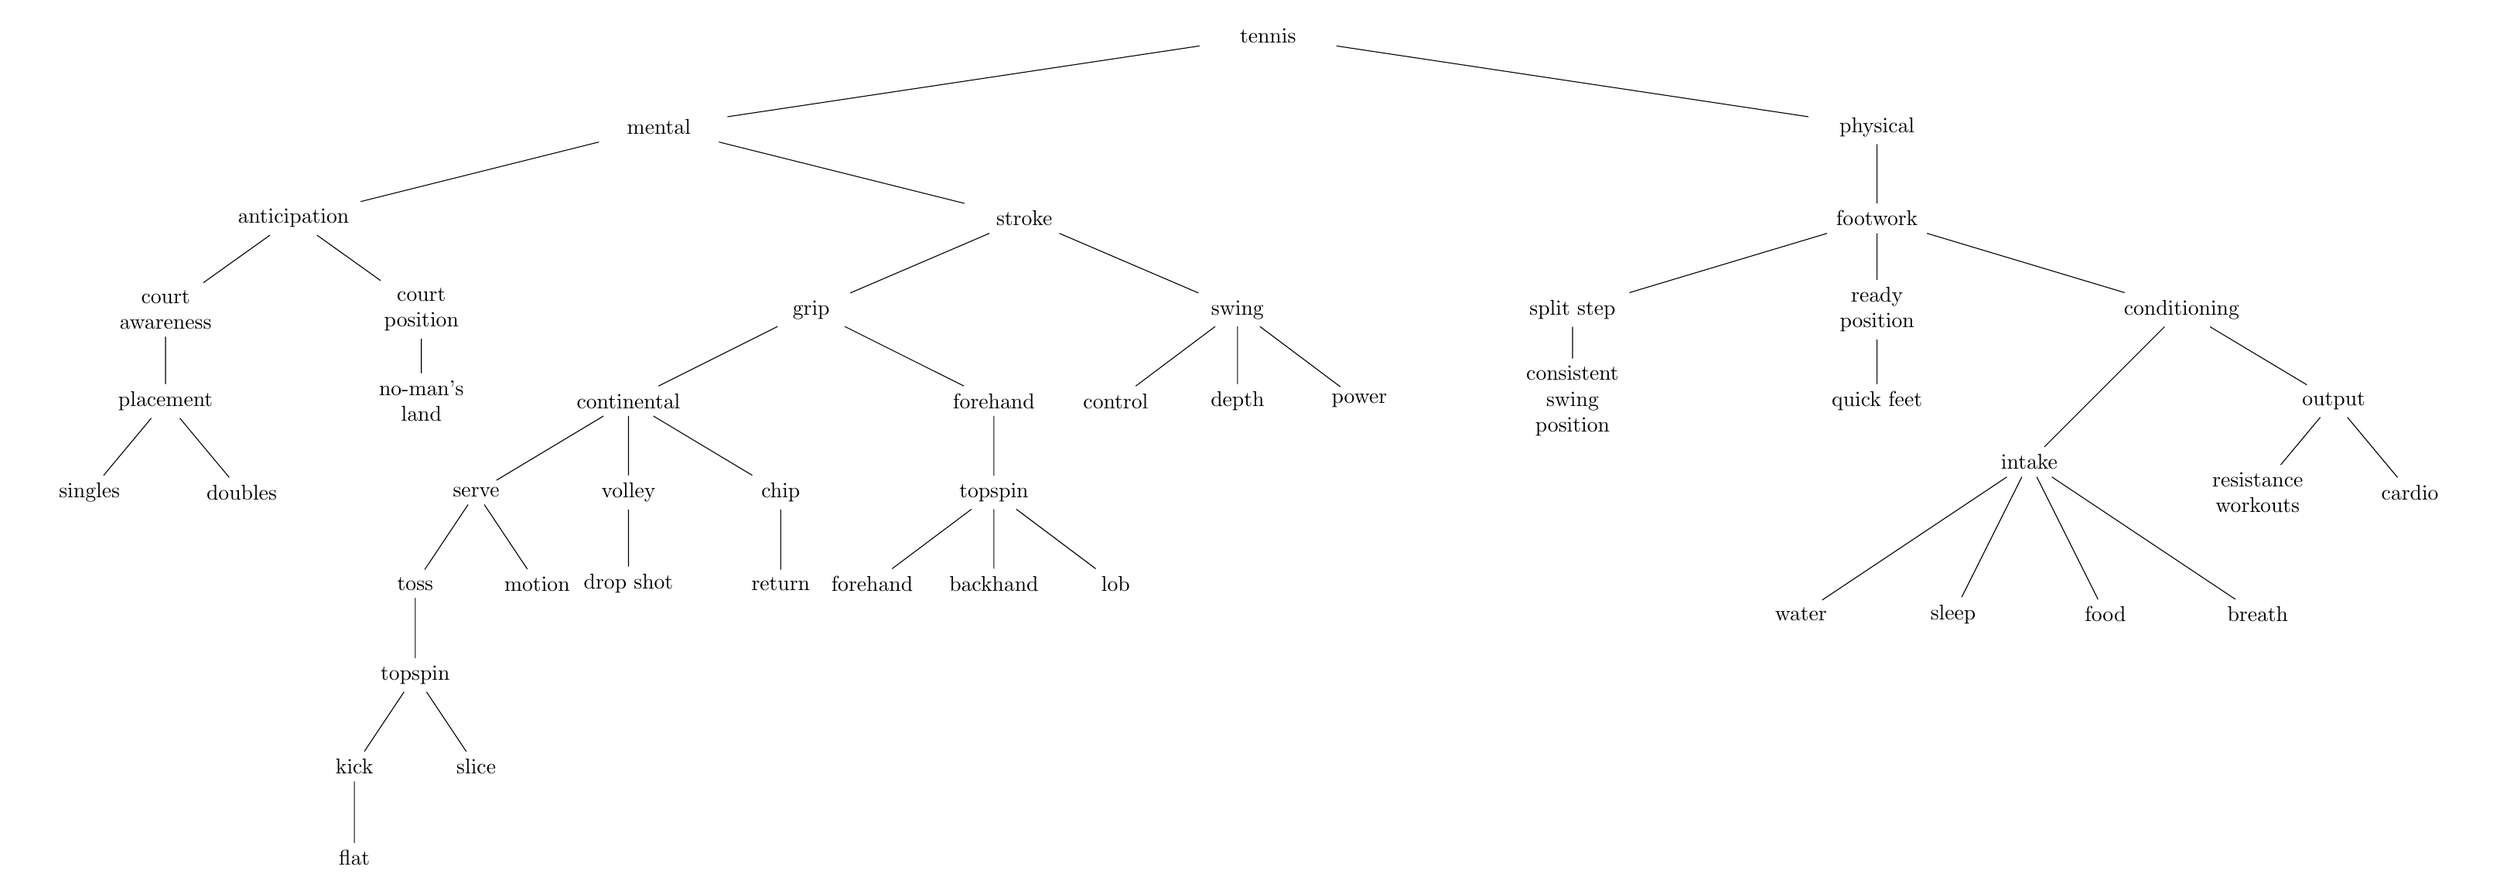
\begin{tikzpicture}[text width=20mm, text centered]

%DISTANCE SETTINGS
\tikzstyle{level 1}=[sibling distance=200mm]
\tikzstyle{level 2}=[sibling distance=120mm]
%\tikzstyle{level 3}=[sibling distance=100mm]
%\tikzstyle{level 4}=[sibling distance=50mm]
\tikzstyle{level 5}=[sibling distance=25mm]
\tikzstyle{level 6}=[sibling distance=20mm]
%\tikzstyle{level 7}=[sibling distance=0mm]
%\tikzstyle{level 8}=[sibling distance=20mm]
%\tikzstyle{level 9}=[sibling distance=0mm]
%NODES
\node {tennis} 
	child {node {mental}
		child {node {anticipation}
			[sibling distance=42mm]
			child {node {court awareness}
				child{node {placement}
					child{node {singles}}
					child{node {doubles}}				
				}			
			}
			child {node {court position}
				child{node {no-man's land}}			
			}
		}
		child {node {stroke}
			[sibling distance=70mm]
			child {node {grip}
				[sibling distance=60mm]
				child {node {continental}
					child {node {serve}
						[sibling distance=20mm]
						child {node {toss}
							child {node {topspin}
								[sibling distance=20mm]
								child {node {kick}
									child {node {flat}}								
								}							
								child {node {slice}}							
							}						
						}
						child {node {motion}}					
					}
					child {node {volley}
						child {node {drop shot}}					
					}
					child {node	{chip}
						child {node {return}}					
					}		
				}
				child {node {forehand}
					child {node {topspin}
						child {node {forehand}}
						child {node {backhand}}
						child {node {lob}}					
					}				
				}
			}							
			child {node {swing}
				[sibling distance=20mm]
				child {node {control}}
				child {node {depth}}
				child {node {power}}			
			}
		}
	}
	child {node {physical}
		child {node {footwork}
		[sibling distance=50mm]
			child {node {split step}
				child {node {consistent swing position}}			
			}
			child {node {ready position}
				child {node {quick feet}}
			}
			child {node {conditioning}				
				child[level distance=25mm] {node {intake}			
					child {node {water}}
					child {node {sleep}}
					child {node {food}}
					child {node {breath}}				
				}
				child {node {output}
					child {node {resistance workouts}}
					child {node {cardio}}				
				}			
			}
		}		
	};
	
\end{tikzpicture}
\end{document}

